\ifspanish

\else

Consider the decision problem with three hypotheses given by likelihood functions
\begin{align*}
p_{X|H}(x|0) &= 2 - 2 x,   \qquad   0 \le x \le 1  \\
p_{X|H}(x|1) &= 1 - \frac12 x,   \qquad   0 \le x \le 2  \\
p_{X|H}(x|2) &= \frac13 - \frac19 x,   \qquad   0 \le x \le 3  \\
\end{align*}
and equal prior probabilities ($P_H(0)=P_H(1)=P_H(2)$).

\begin{parts}
\part Compute the decision regions of the ML classifier
\part Compute the probability of deciding $D=2$ knowing that the true hypothesis is $H=1$.
\part Consider the binary decision problem given by two hypothesis:
\begin{align*}
H' &= 0:  \qquad H=0        \\
H' &= 1:  \qquad H \neq 0 
\end{align*}
Compute the ML classifier.
%\part Compute the false alarm probability.
\end{parts}

\begin{solution}
\begin{parts}
\part The figure shows the likelihood functions.
\begin{center}
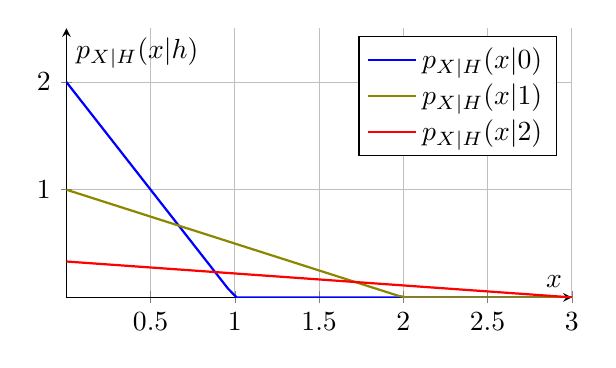
\begin{tikzpicture}
\begin{axis}[
    xlabel={$x$},
    ylabel={$p_{X|H}(x|h)$},
    xmin=0, xmax=3,
    ymin=0, ymax=2.5,
    axis lines=middle,
    legend pos=north east,
    grid=both,
    width=8cm,
    height=5cm,
    every axis plot/.append style={thick}]
\addplot[domain=0:5, samples=100, blue] {max(2 - 2*x, 0)};
\addlegendentry{$p_{X|H}(x|0)$}
\addplot[domain=0:5, samples=100, olive] {max(1 - 0.5*x, 0)};
\addlegendentry{$p_{X|H}(x|1)$}
\addplot[domain=0:5, samples=500, red] {max(1/3 - x / 9, 0)};
\addlegendentry{$p_{X|H}(x|2)$}
\end{axis}
\end{tikzpicture}
\end{center}

The boundary decision will be the solutions of
\begin{align*}
\begin{array}{lll}
2-2x = 1-\frac{1}{2} x            & \Rightarrow   & x = \frac23  \\
1-\frac12 x = \frac13-\frac19 x   & \Rightarrow   & x = \frac{12}7  
\end{array}
\end{align*}
Therefore, the decision regions are
\begin{align*}
\boxed{{\cal X}_0 = \left[0,          \frac23   \right]},  \qquad
\boxed{{\cal X}_1 = \left[\frac23,    \frac{12}7   \right]},  \qquad
\boxed{{\cal X}_2 = \left[\frac{12}7, 3            \right]}
\end{align*}

\part
\begin{align*}
P\{D=2|H=1\} = \int_{{\cal X}_2} p_{X|H}(x|1) dx  
             = \int_{\frac{12}{7}}^2 (1 - 0.5 x) dx 
             = \left[x - \frac14 x^2\right]_{\frac{12}{7}}^2
             = \frac{1}{49}
\end{align*}
\part
The likelihood functions for this problem are
\begin{align*}
p_{X|H'}(x|0) &= p_{X|H}(x|0) = 2 - 2 x,   \qquad   0 \le x \le 1  \\
p_{X|H'}(x|1) &= p_{X|H',H}(x|1,0) P_{H|H'}(1|0) + p_{X|H',H}(x|1,1) P_{H|H'}(1|1) + p_{X|H',H}(x|1,2) P_{H|H'}(1|2)   \\
              &= \frac12 p_{X|H',H}(x|1,1) + \frac12 p_{X|H',H}(x|1,2)   \\
              &= \left[\begin{array}{ll}
                       \frac23 - \frac{11}{36} x,    &   0 \le x \le 2    \\
                       \frac16 - \frac1{18} x,       &   2 \le x \le 3
                       \end{array}
                 \right]
\end{align*}
The ML classifier will be will
\begin{align*}
p_{X|H'}(x|1) \dunodcero p_{X|H'}(x|0)  
	& \quad \Leftrightarrow \quad \frac23 - \frac{11}{36} x \dunodcero 2 - 2 x   \\
	& \quad \Leftrightarrow \quad \frac{61}{36} x \dunodcero \frac43       \\
	& \quad \Leftrightarrow \quad x \dunodcero \frac{48}{61}     
\end{align*}

\end{parts}
\end{solution}

\fi